\documentclass[../paper.tex]{subfiles}
\begin{document}
\section{Production}
\label{sec:production}

\subsection{Data Augmentation}
For the semantic gloss-to-pose retrieval step, we extracted skeletal poses from sign language videos using Google MediaPipe Holistic \cite{MediaPipe}. Furthermore, we used the all-MiniLM-L6-v2 embedding model \cite{minilm} to embed the glosses, and then stored the embeddings, glosses, and corresponding poses in a pgvector PostgreSQL database. This process allowed us to semantically retrieve and stitch together pose sequences for inputted gloss sequences.

\subsection{Inference}
The inference stage of the sign language production component includes two main steps: text-to-gloss translation and semantic gloss-to-pose retrieval. \autoref{fig:production_flow} demonstrates the complete inference architecture of the pose retrieval component of the interface.

\begin{figure}[!htbp]
  \centerline{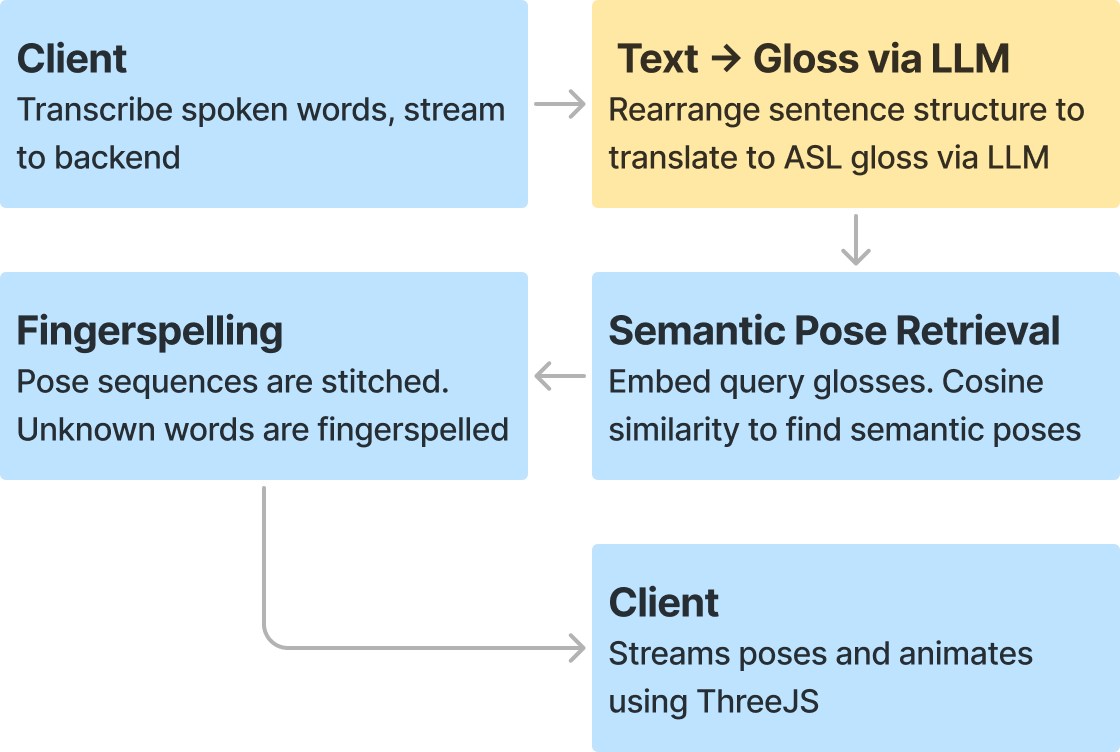
\includegraphics[width=\linewidth]{../figures/production-flow.png}}
  \caption{Complete pose-retrieval infrastructure}\label{fig:production_flow}
\end{figure}

\subsubsection*{Text \textrightarrow\ Gloss Translation} We use a large language model (LLM) to translate spoken English text to ASL gloss. The LLM is instructed with a rule-based prompt which guides the model to generate ASL gloss by dropping articles and rearranging subjects, objects, and verbs. In the deployed interface, we use OpenAI's GPT-4o \cite{gpt4o} model because of its inference speed and accuracy. Alternative open-source LLMs can be easily integrated into the interface.
\subsubsection*{Semantic Gloss \textrightarrow\ Pose Retrieval}
The gloss sequences from the previous step are now individually embedded using the all-MiniLM-L6-v2 embedding model. These query vectors are used to semantically query the pgvector database with a certain cosine similarity threshold, allowing us to retrieve and stitch together contextually-similar pose sequences for inputted gloss sequences. For glosses that do not meet our cosine similarity threshold, we simply stitch together the poses of fingerspelling letters, allowing for the generation of poses for glosses not present in the data set.
\end{document}